\section{Event and Object Selection}
\label{sec:AN_Selection}

%In this chapter we document the electron, muon, and photon identification and isolation criteria, $E_T^{MET}$ criteria, and provide the results of comparing simulation with data.
\subsection{Object Selection}
\label{sec:AN_ObjectSelection}

We select events with a muon and a photon in the final state for the muon channel and events with an electron and a photon in the final state for the electron channel. 

We apply selection requirements on transverse momenta of $P_T^{\mu}>25$ GeV on muons,  $P_T^e>30$~GeV on electrons and $P_T^{\gamma}>15$~GeV on photons. In addition, electrons and photons must be within barrel (EB) or endcap (EE) sections of the Ecal which correspondto pseudorapidity ranges of $|\eta^{e,\gamma}| < 1.4442$ and $1.566 < |\eta^{e,\gamma}| < 2.5$, respectively. Muons must be within $|\eta^{\mu}|<2.1$. Selection requirements on $P_T^{\mu}$, $\eta^{\mu}$, and $P_T^e$ are determined by the trigger requirements, $\eta^{e,\gamma}$ criteria are determined by the geometrical limitations of the detector acceptance, and $P_T^{\gamma}>15$~GeV is the phase space requirement.

CMS Particle Object Group (POG) provides their recommendations for object identification~(ID) criteria for any given period of data collection. Recommendations for~2012 data include two sets of muon~ID criteria: "Tight" and "Loose" and four sets of electron and photon~ID criteria: "Tight", "Medium", "Loose" and "Veto".

For muon selection, we apply "Tight"~ID criteria. We consider electrons passing the "Tight" ID criteria and photons passing the modified "Medium" ID criteria. The modification of the photons ID criteria was studied in the $W\gamma\gamma \rightarrow l\nu\gamma\gamma$ measurement~\cite{ref_Wgg8TeV}.  %No restrictions on the maximum number of the final state photons are applied, however, 

To reduce backgrounds from the process with two or more leptons, such as $Z\gamma\rightarrow l l \gamma$ process, in the muon channel, we reject all events that have the second reconstructed muon candidate with $P_T^{\mu}>10$ GeV and $|\eta|^{\mu}<2.4$, and in the electron channel, we reject events which have the second reconstructed electron candidate with $p_T^e>10$ GeV and satisfying the "Veto"~ID criteria.

Selection criteria are applied consistently on the data sample as well as on all MC samples. The selection efficiency may differ between data and MC. The ratios data and MC efficiencies are called the scale factors. The scale factors for the selection criteria recommended are provided by CMS POG. For the modified photon~ID criteria, the appropriate changes to the POG-recommended scale factors were applied derived by the $W\gamma\gamma$ team~\cite{ref_Wgg8TeV}.

\subsection{Event Level Selection}
\label{sec:AN_Selection_EventLevel}

In the final state of the $W\gamma\rightarrow l\nu\gamma$ process, there is a lepton, a photon, and a neutrino. Because of that, we select events with exactly one lepton (muon or electron), a photon, both originating from the primary vertex, and with the significant missing transverse energy $E_T^{miss}$. The selection criteria for the individual electrons, muons and photons are described in Ch.~\ref{sec:AN_ObjectSelection}.

To select events with significant $E_T^{miss}$, we introduce a selection requirement on the transverse mass of a $W$~boson $M_T^W$ which is related to $E_T^{miss}$ as: 
\begin{equation}
M_T^W=\sqrt{(2  P_T^{l}  E_T^{miss}  (1-\cos{(\phi^{l}-\phi^{miss})}))},
\end{equation}
\noindent{where $P_T^l$ is a lepton transverse momentum, $\phi^{l}$ is an azimuthal angle of the lepton momentum, and $\phi^{miss}$ is an azimuthal angle of the missing transverse momentum. The requirement is $M_T^W>40$~GeV. The $M_T^W$ distribution is shown in Fig.~\ref{fig:DATAvsMC_WMt}. Photons with $P_T^{\gamma}<45$~GeV are selected for this plot because for such photons we do not expect them to be result of a new physics process.}

After the listed selection criteria are applied, significant background from DY+jets in the electron channel remains. This background is caused by one of the electrons misidentified as a photon. Its contribution is the most significant around the invariant mass of the electron-photon system $M_{e\gamma}$ close to the mass of the $Z$ boson (Fig.~\ref{fig:DATAvsMC_Mpholep1})because the distribution of $M_{ee}$ in the $Z\rightarrow e e$ decay is peaking at the value of the Z boson mass. To reduce this background, we apply $Z$-mass window selection criterion, more specifically, events with $70$~GeV$<M_{e\gamma}<110$~GeV are rejected. 

Finally, the separation $\Delta R=\sqrt{({\Delta\phi}^2+{\Delta\eta}^2)}$ between the final state lepton and photon is required to be $\Delta R(l,\gamma)>0.7$ to enhance the TGC contribution. In case if there is more than one photon in the selected event, the candidate with the photon of the highest~$P_T^{\gamma}$ is selected. 

Data and MC in Fig.~\ref{fig:DATAvsMC_WMt}-\ref{fig:DATAvsMC_Mpholep1} significantly disagree. Thus, a data-driven method is necessary to estimate the backgrounds.

\begin{figure}[htb]
  \begin{center}
   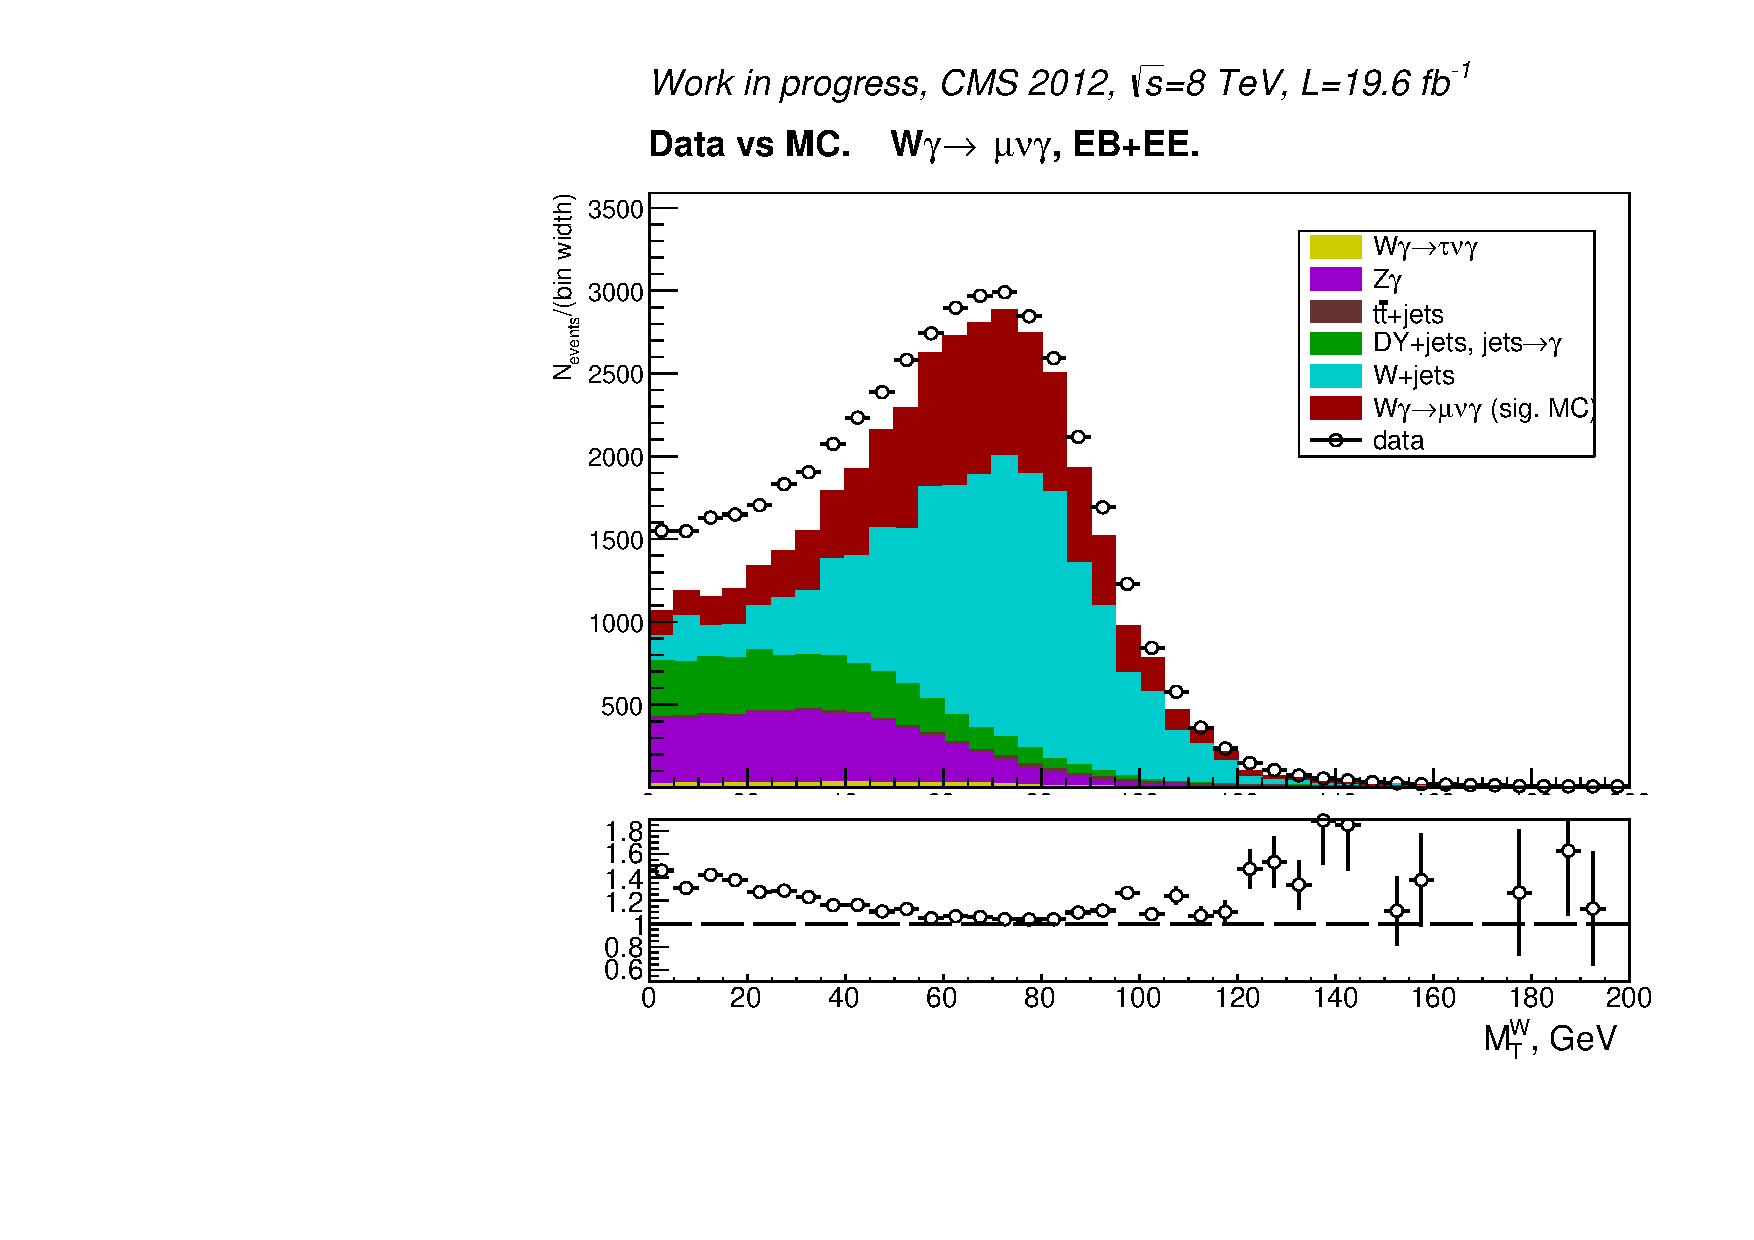
\includegraphics[width=0.5\textwidth]{../figs/figs_v11/MUON_WGamma/PrepareYields/c_TotalDATAvsMC_EtaCommon__WMtVERY_PRELIMINARY.pdf}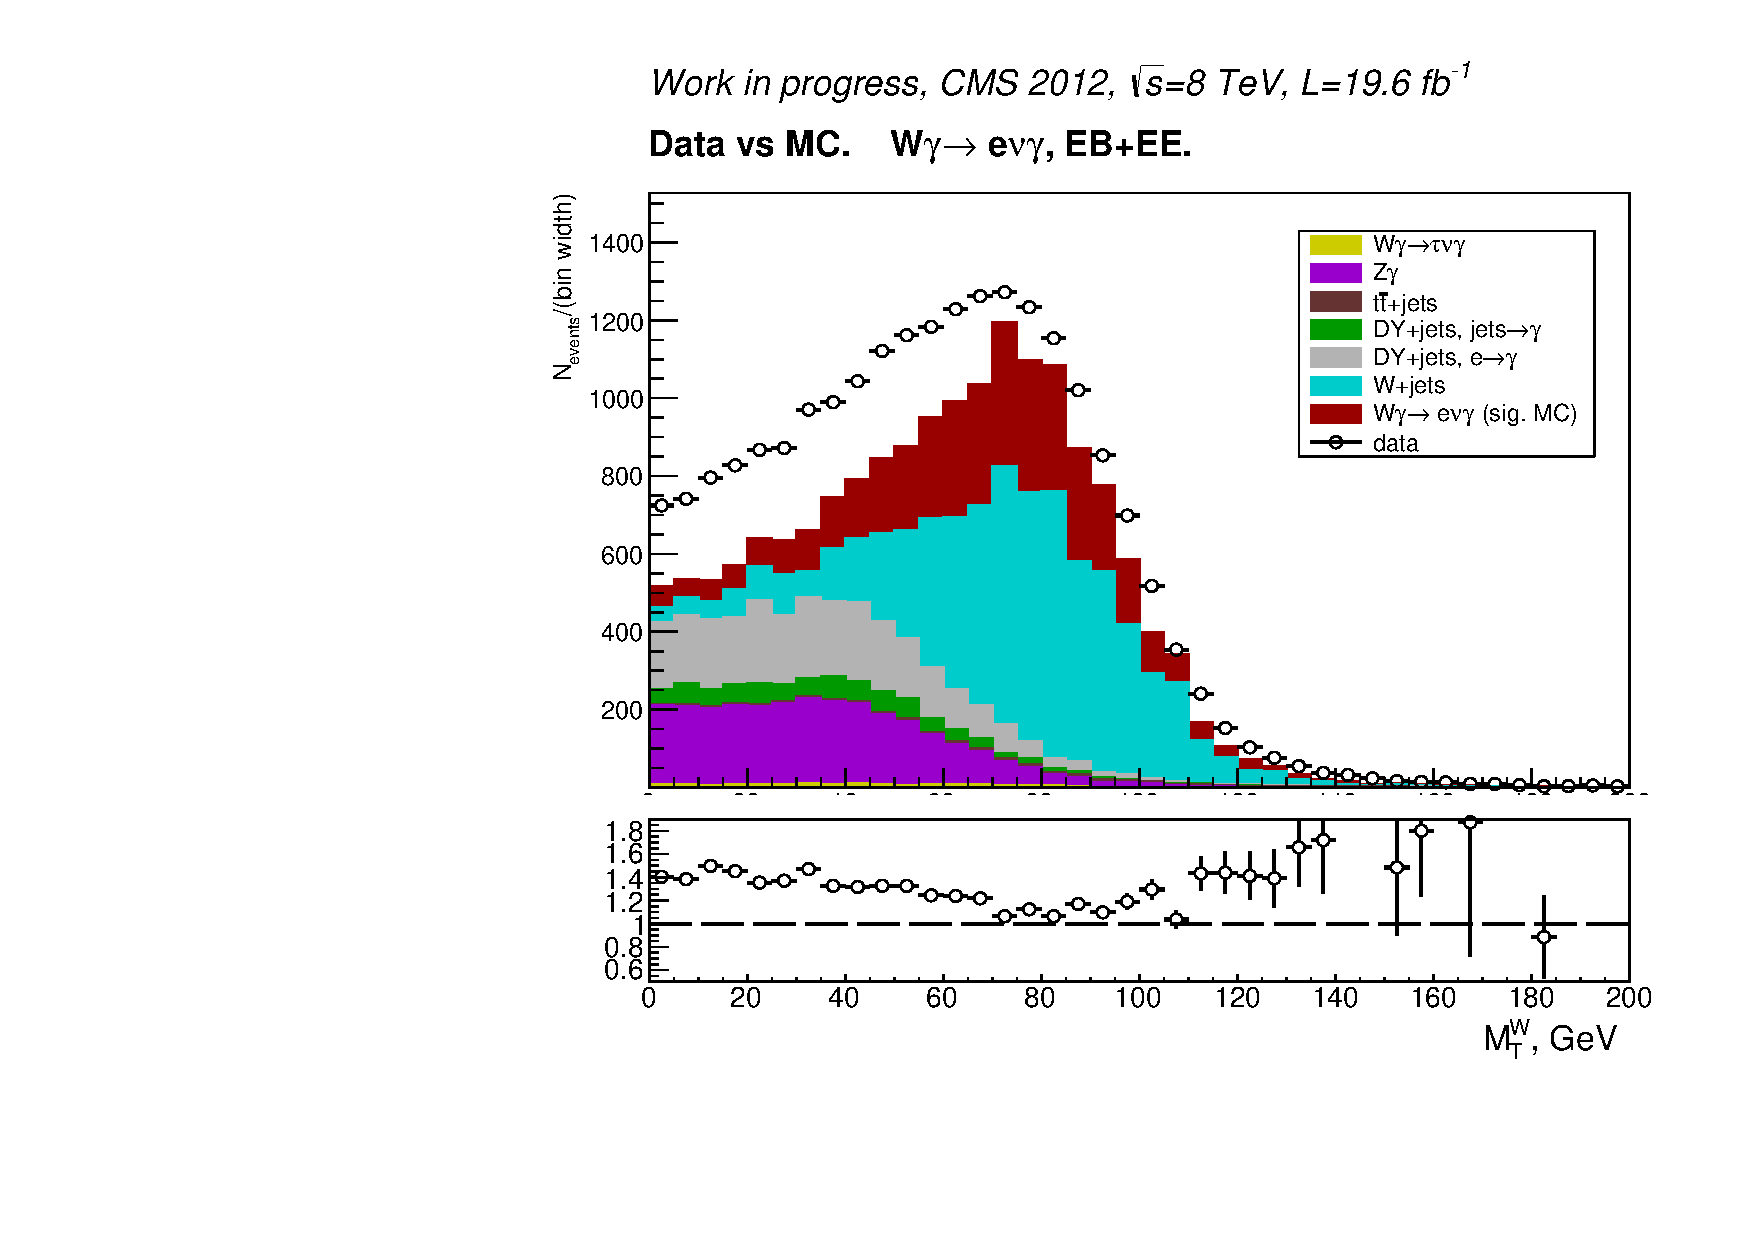
\includegraphics[width=0.5\textwidth]{../figs/figs_v11/ELECTRON_WGamma/PrepareYields/c_TotalDATAvsMC_EtaCommon__WMtVERY_PRELIMINARY.pdf}
  \caption{ $M_T^W$ of $W\gamma$ candidates. Data vs MC plots. Left: muon channel, right: electron channel. All selection criteria except $M_{T}^W$ cut are applied on these plots. $15$~GeV$<P_T^{\gamma}<45$~GeV. }
  \label{fig:DATAvsMC_WMt}
  \end{center}
\end{figure}

\begin{figure}[htb]
  \begin{center}
   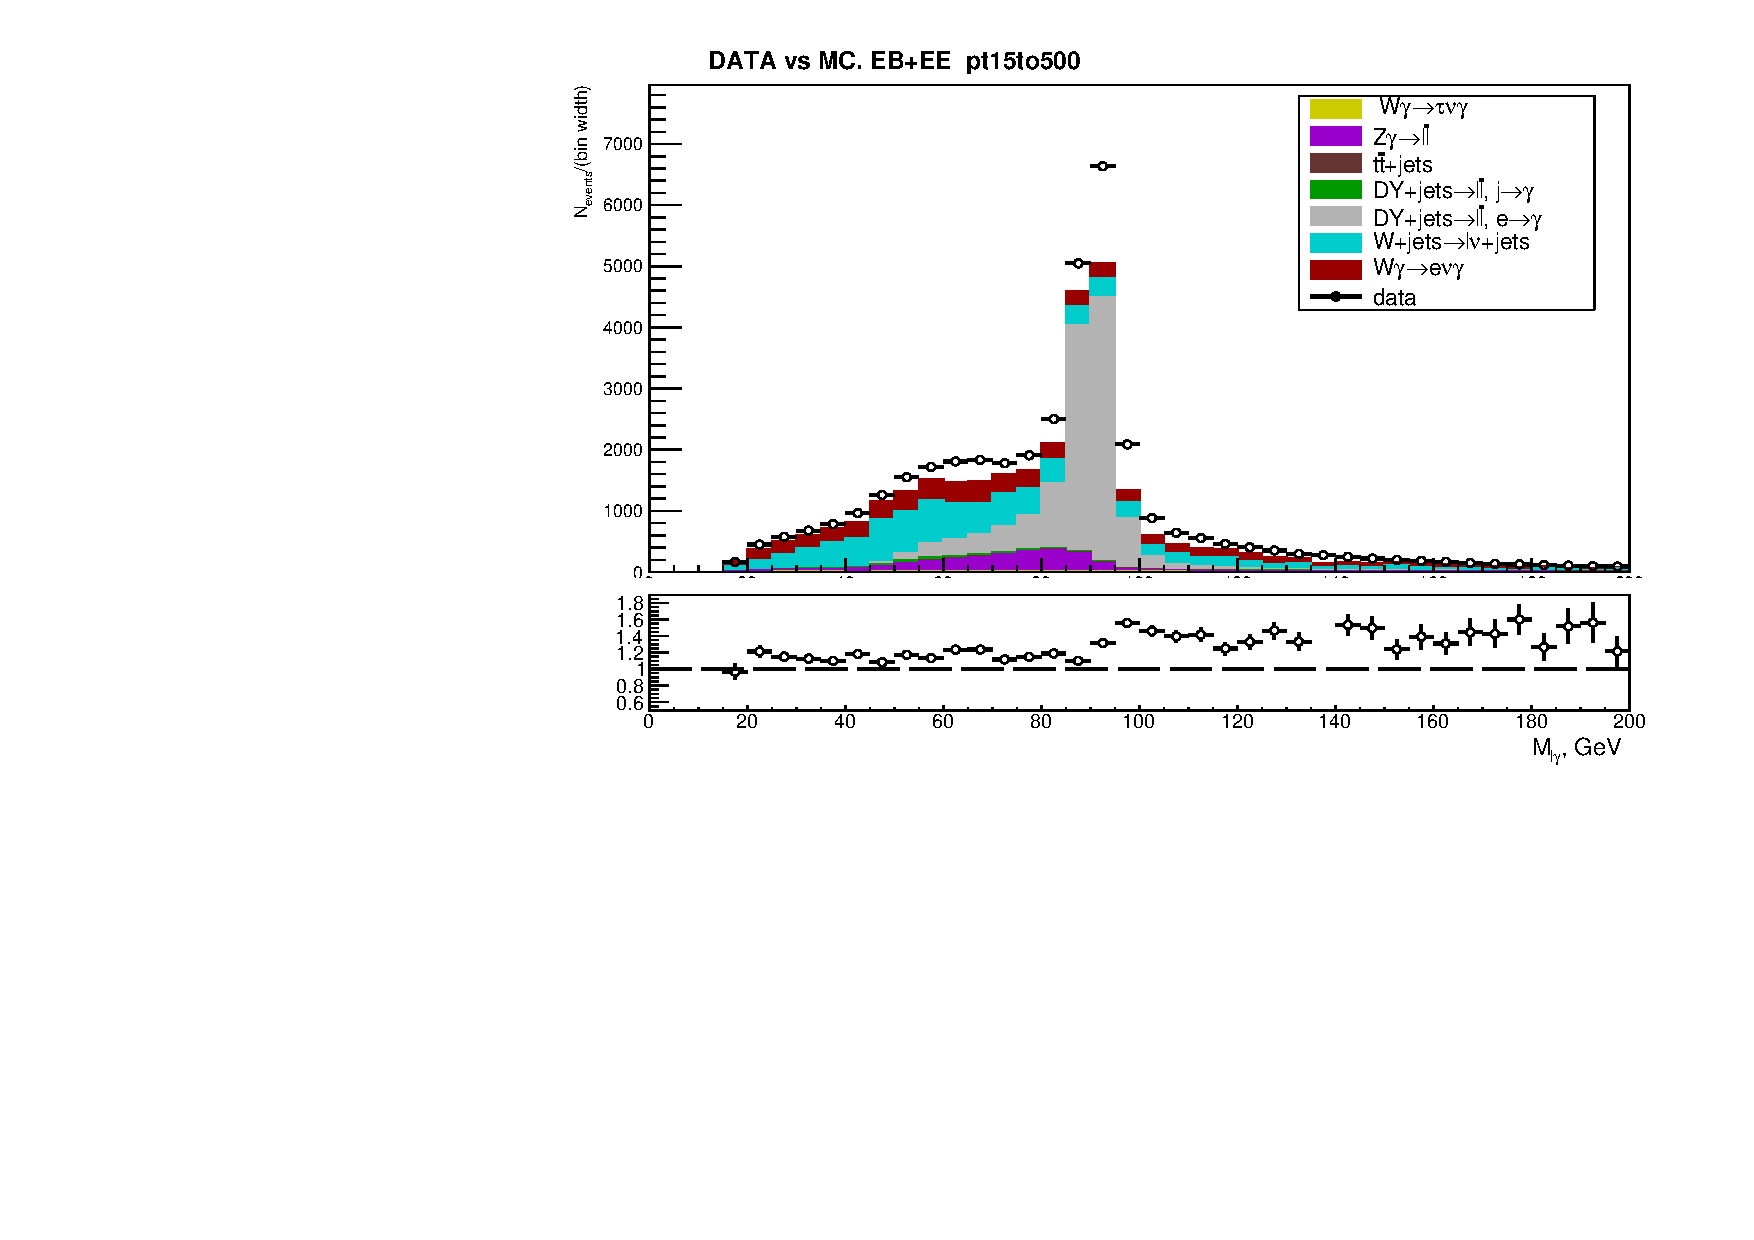
\includegraphics[width=0.7\textwidth]{../figs/figs_v11/ELECTRON_WGamma/PrepareYields/c_TotalDATAvsMC_EtaCommon__Mpholep1PRELIMINARY_FOR_E_TO_GAMMA_WITH_PSV_CUT_pt15to500_.pdf}
  \caption{$M_{l\gamma}$ of $W\gamma$ candidates in the electron channel. Data vs MC plots. All selection criteria except $Z$-mass window are applied on this plot. $P_T^{\gamma}>15$~GeV. }
  \label{fig:DATAvsMC_Mpholep1}
  \end{center}
\end{figure}

In addition to $W\gamma$-selected datasets, we also prepare $Z\gamma$-selected datasets which are used for background estimation (Ch.~\ref{sec:BackgroundSubtraction}) and for cross checking (App.~\ref{sec:ZgCheck}). We select $Z\gamma$ events in muon and electron channels. Selection requirements include at least two muons (or electrons) and at least one photon in the final state. Kinematis and identification requirements on the objects are the same as for the $W\gamma$ selection. Unlike in $W\gamma$, in $Z\gamma$ selection in the electron channel, photons are required to pass ``Medium'' ID without any modifications. Invariant mass of the final state lepton pair is required to be $M_{ll}>50$~GeV. Finally, a separation between photon and each lepton must be $\Delta R>0.7$. 

\subsection{Selected Events}

%Distributions of $P_T^{\gamma}$ and $M_T^W$ of the selected events are shown in Fig. \ref{fig:DATAvsMC} and \ref{fig:DATAvsMC_WMt}. 
%The is a large discrepancies in all the distributions and therefore the data-driven background estimates are necessary.\\

Distributions of $P_T^{\gamma}$ of the selected events are shown in Fig.~\ref{fig:DATAvsMC}. The are large discrepancies in all the distributions and therefore the data-driven background estimates are necessary.

\begin{figure}[htb]
  \begin{center}
   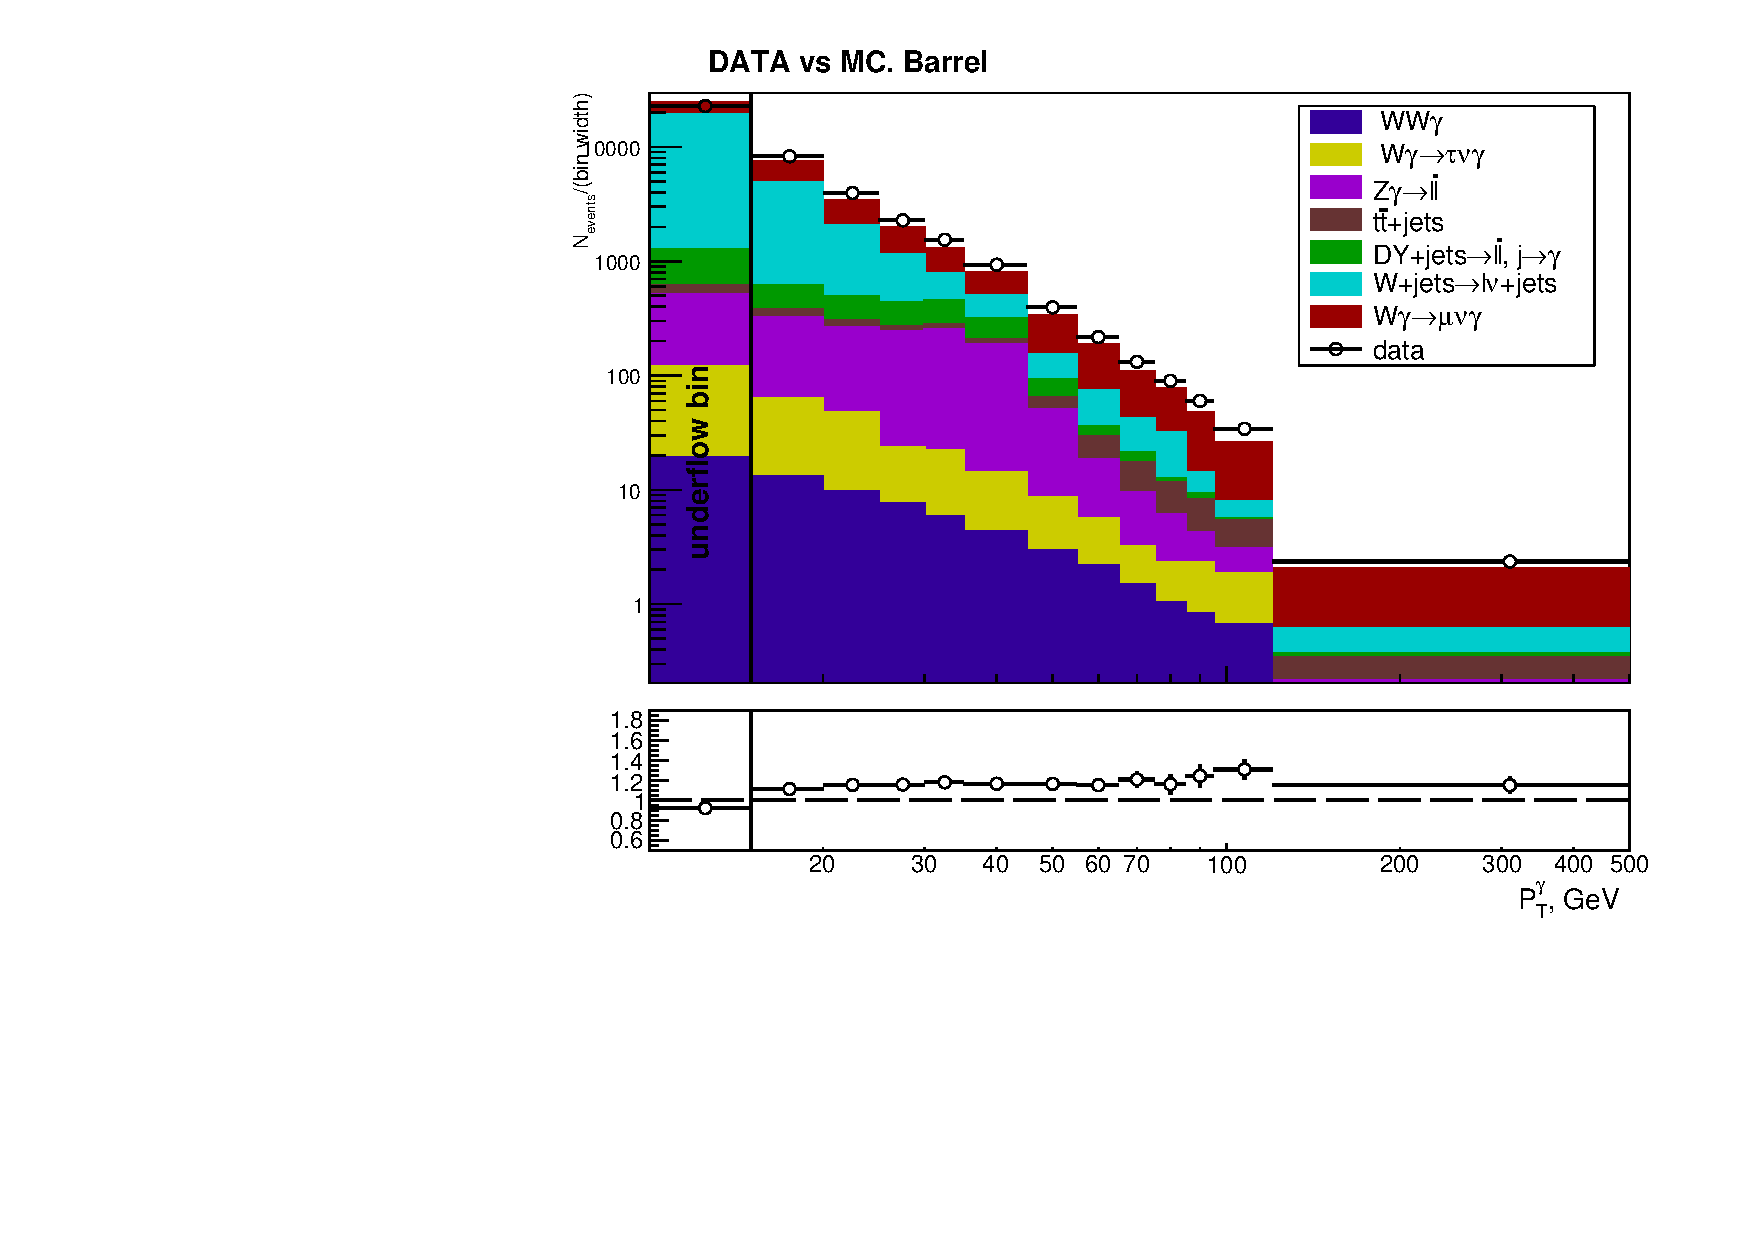
\includegraphics[width=0.45\textwidth]{../figs/figs_v11/MUON_WGamma/PrepareYields/c_TotalDATAvsMC_Barrel__phoEt.pdf}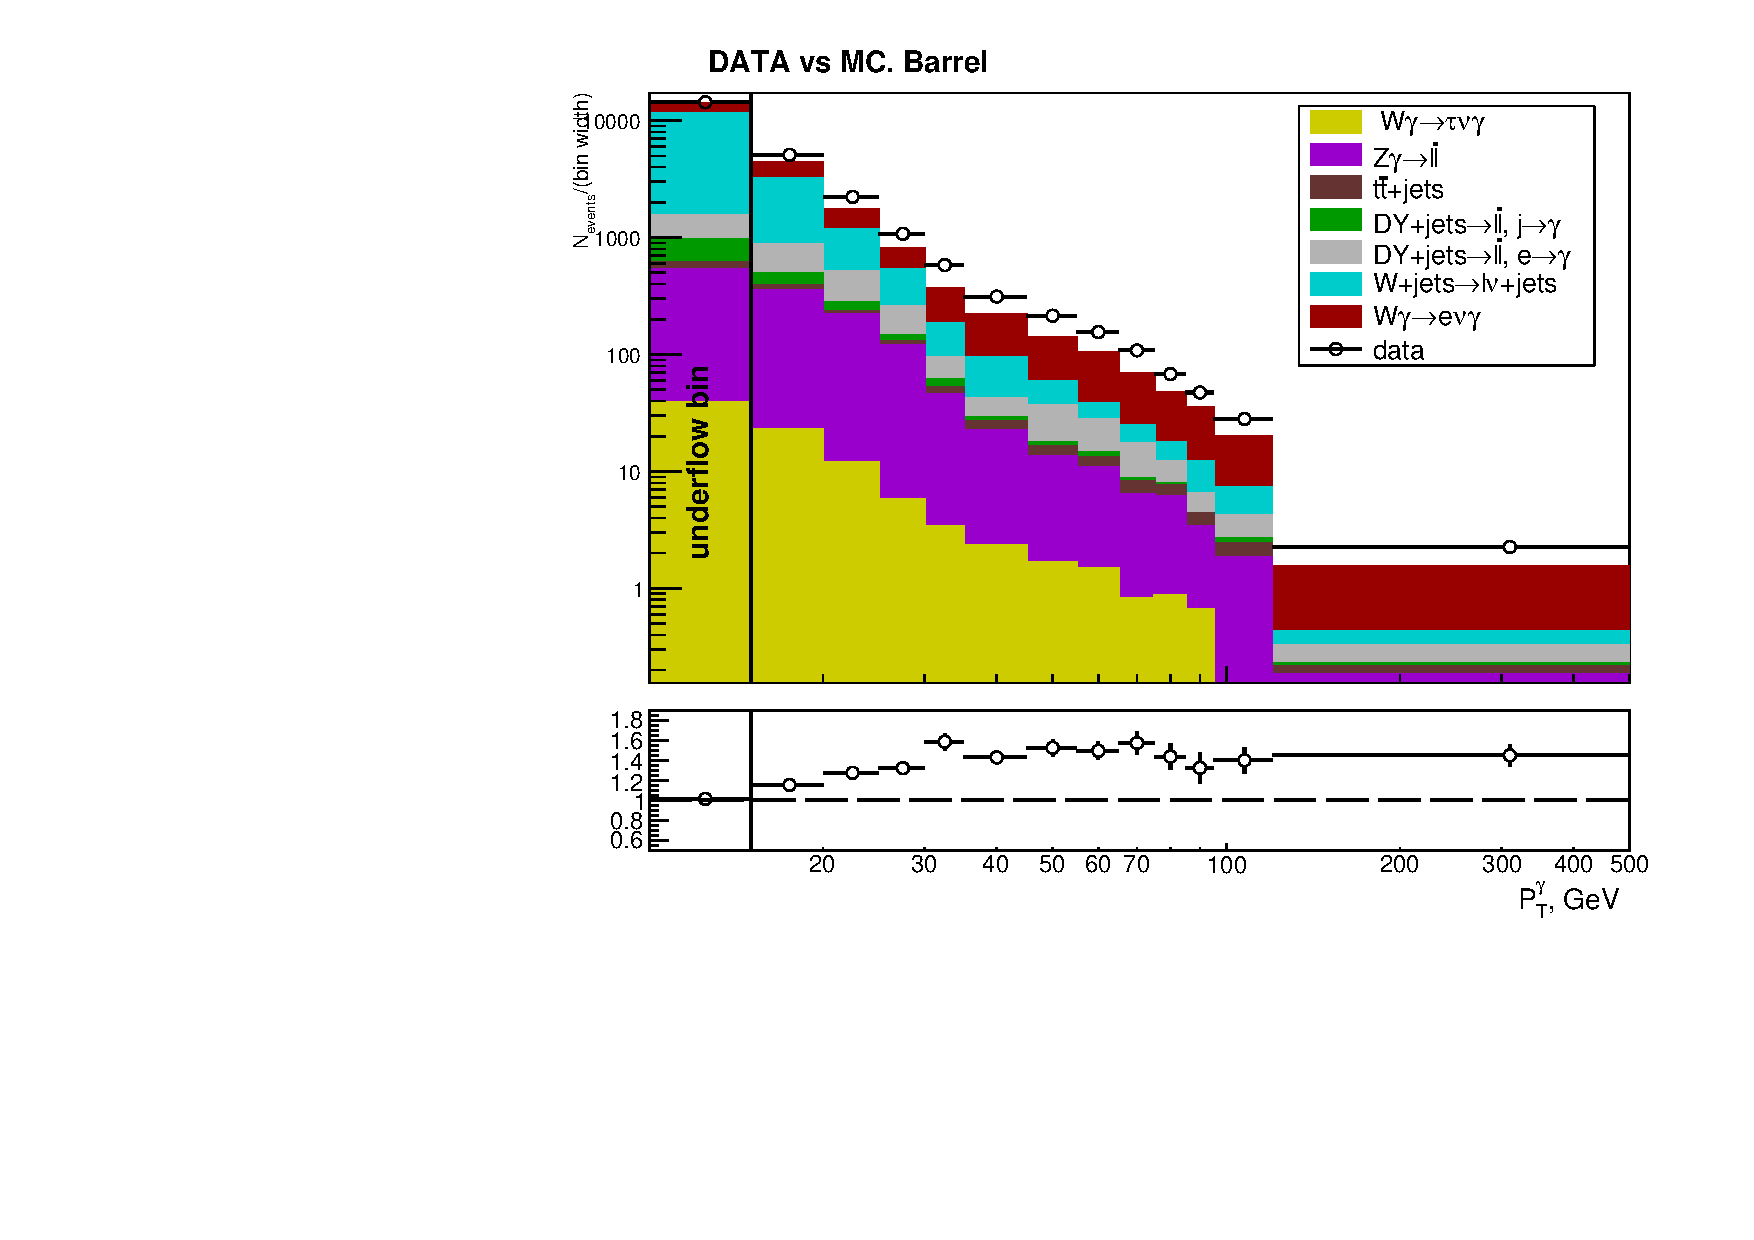
\includegraphics[width=0.45\textwidth]{../figs/figs_v11/ELECTRON_WGamma/PrepareYields/c_TotalDATAvsMC_Barrel__phoEt.pdf}
   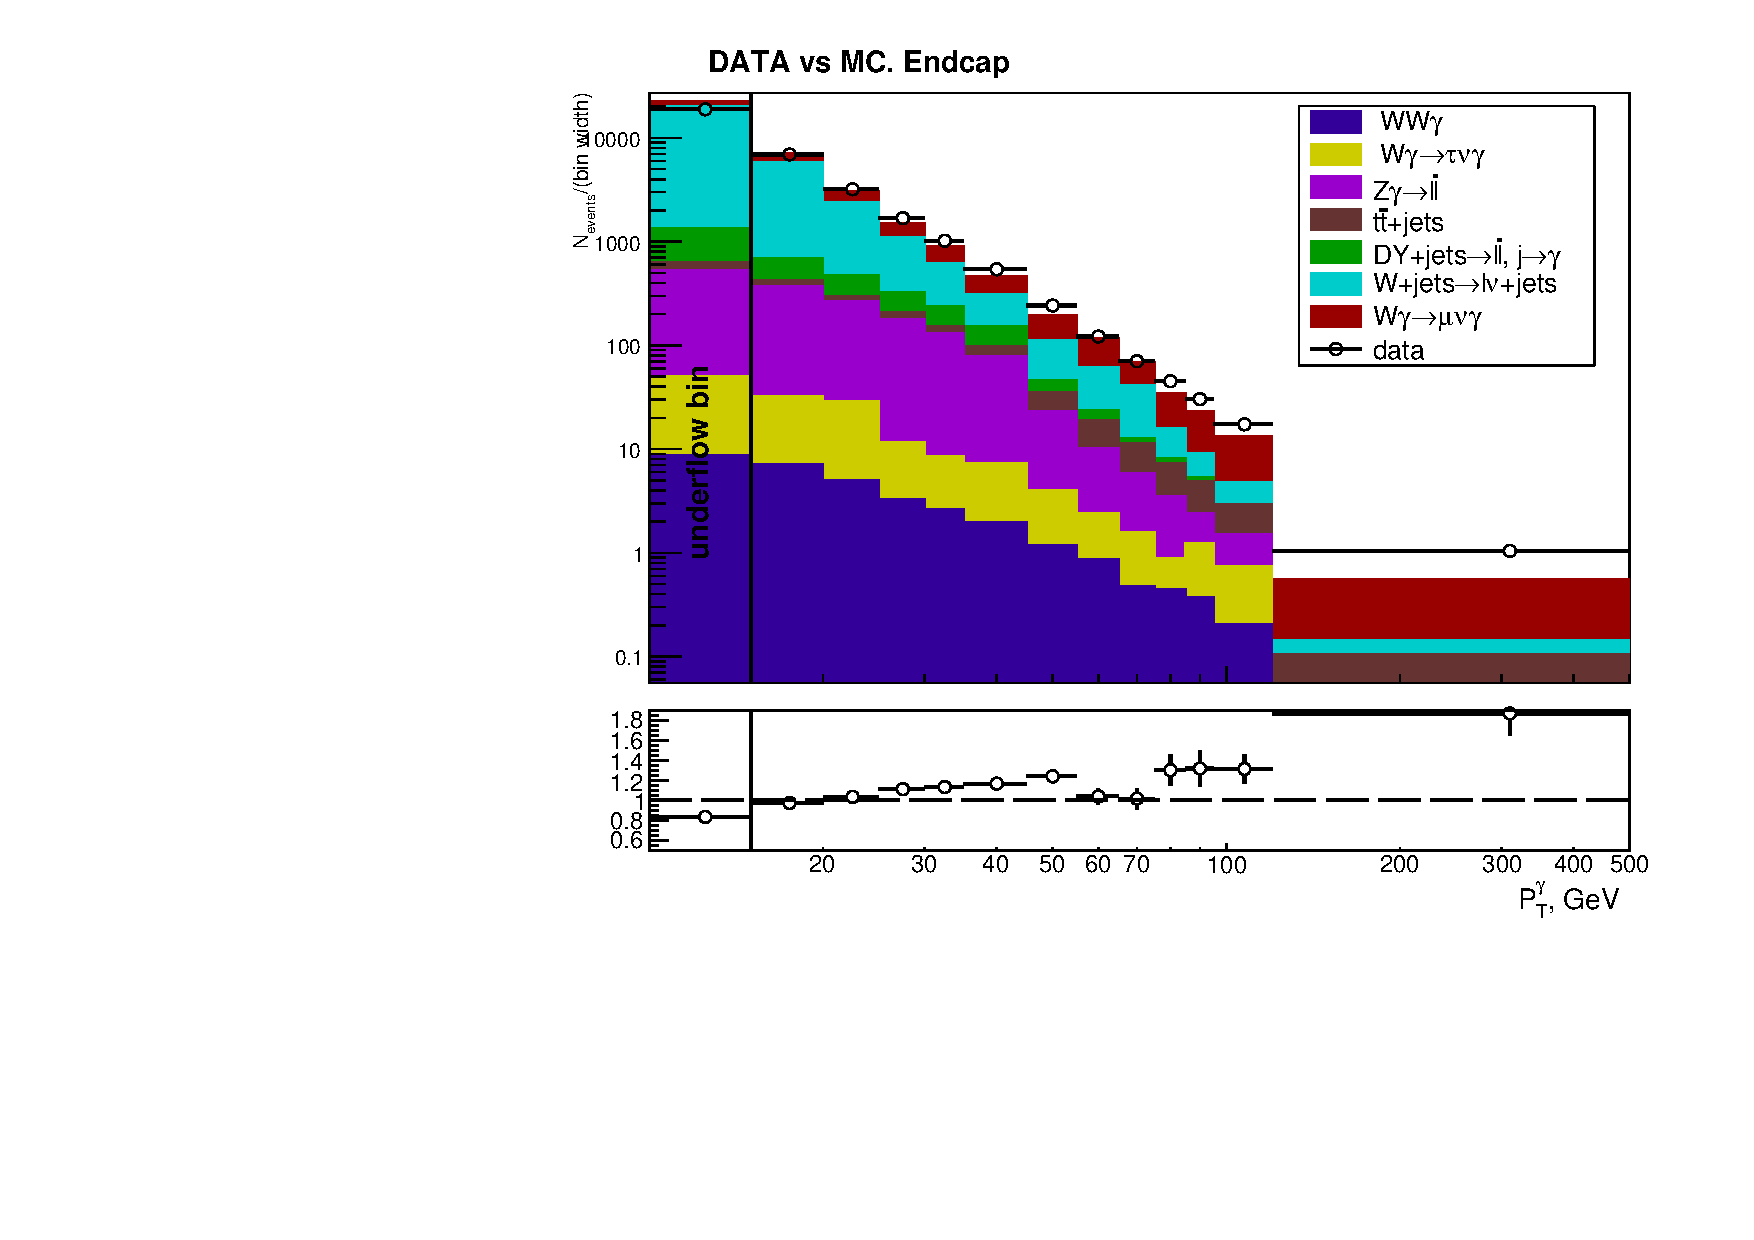
\includegraphics[width=0.45\textwidth]{../figs/figs_v11/MUON_WGamma/PrepareYields/c_TotalDATAvsMC_Endcap__phoEt.pdf}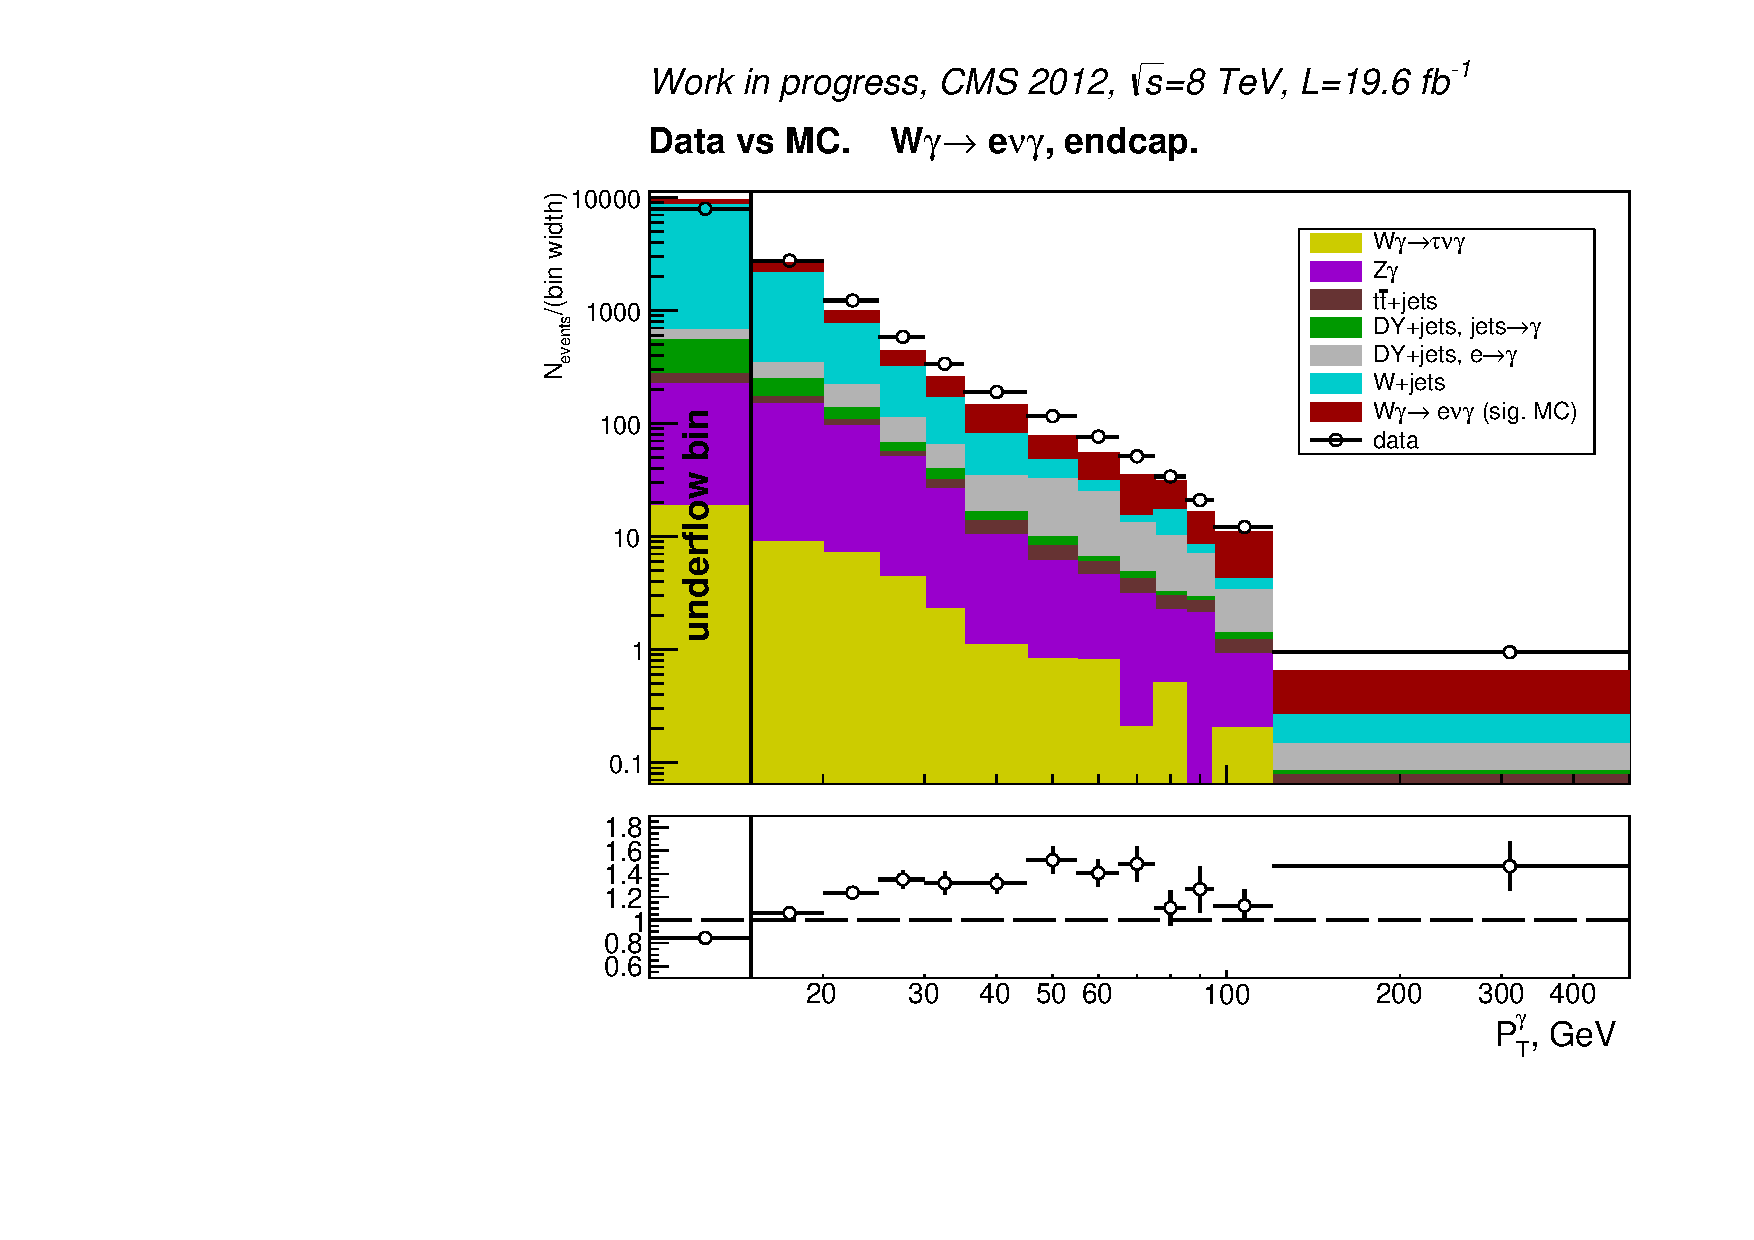
\includegraphics[width=0.45\textwidth]{../figs/figs_v11/ELECTRON_WGamma/PrepareYields/c_TotalDATAvsMC_Endcap__phoEt.pdf}
  \caption{$P_T^{\gamma}$ of $W\gamma$ candidates. Data vs MC plots. Left column: muon channel, right column: electron channel. Top to bottom: photons in EB and EE of ECal.}
  \label{fig:DATAvsMC}
  \end{center}
\end{figure}



%\begin{figure}[htb]
%  \begin{center}
%   \includegraphics[width=0.45\textwidth]{figs_v8/MUON_WGamma/PrepareYields/c_TotalDATAvsMC_Barrel__WMtVERY_PRELIMINARY.pdf}\includegraphics[width=0.45\textwidth]{figs_v8/ELECTRON_WGamma/PrepareYields/c_TotalDATAvsMC_Barrel__WMtVERY_PRELIMINARY.pdf}
%   \includegraphics[width=0.45\textwidth]{figs_v8/MUON_WGamma/PrepareYields/c_TotalDATAvsMC_Endcap__WMtVERY_PRELIMINARY.pdf}\includegraphics[width=0.45\textwidth]{figs_v8/ELECTRON_WGamma/PrepareYields/c_TotalDATAvsMC_Endcap__WMtVERY_PRELIMINARY.pdf}
%  \caption{Data vs MC plots, $M_T^W$. Left column - muon channel, right column - electron. Top to bottom: barrel and endcap photons. All selection criteria except $M_T^W$ cut on these plots. $15$~GeV$<P_T^{\gamma}<45$~GeV. The analysis cut of $M_T^W>40$~GeV is selected.}
%  \label{fig:DATAvsMC_WMt}
%  \end{center}
%\end{figure}
